\documentclass[tikz,border=3pt]{standalone}

\begin{document}

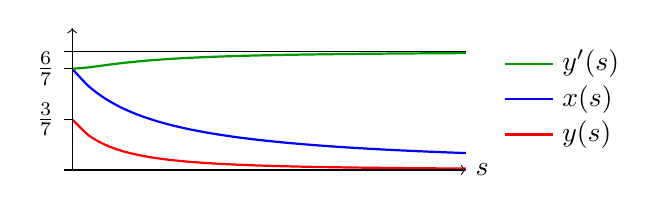
\begin{tikzpicture}[yscale=1.5]

% ===== グラフ部分だけクリップ =====
\begin{scope}
  \clip (0,0) rectangle (5,1);

  % x(s)
  \draw[domain=0:5, smooth, variable=\s, blue, thick]
    plot ({\s}, {6/7*(1+\s)^(-1)});

  % y(s)
  \draw[domain=0:5, smooth, variable=\s, red, thick]
    plot ({\s}, {3/7*(1+\s)^(-2)});

  % y'(s)
  \draw[domain=0:5, smooth, variable=\s, green!60!black, thick]
    plot ({\s}, {
      1 - 6/7*(0.5*(1+\s)^(-2) - (1/3)*(1+\s)^(-3))
    });
\end{scope}

% ===== 軸 =====
\draw[->] (0,0) -- (5,0) node[right] {$s$};
\draw[->] (0,0) -- (0,1.2);

% y = 1 の線
\draw (0,1) -- (5,1);

% 縦軸の目盛り
\draw (0,0) -- (-0.1,0) node[left] {};
\draw (0,{3/7}) -- (-0.1,{3/7}) node[left] {$\frac{3}{7}$};
\draw (0,{6/7}) -- (-0.1,{6/7}) node[left] {$\frac{6}{7}$};
\draw (0,1) -- (-0.1,1) node[left] {};

% ===== 凡例（グラフ外） =====
\begin{scope}
  \draw[green!60!black, thick] (5.5,0.9) -- (6.1,0.9);
  \node[right] at (6.1,0.9) {$y'(s)$};
  
  \draw[blue, thick] (5.5,0.6) -- (6.1,0.6);
  \node[right] at (6.1,0.6) {$x(s)$};

  \draw[red, thick] (5.5,0.3) -- (6.1,0.3);
  \node[right] at (6.1,0.3) {$y(s)$};
\end{scope}

\end{tikzpicture}

\end{document}